\chapter{Evaluation}
%Sandra
\Autor{Sandra Schröder}\\\\
In diesem Kapitel werden die beiden entwickelten Algorithmen gegenüber gestellt. Zwei zentrale Kriterien zur Evaluation der Algorithmen werden thematisiert.
\begin{itemize}
\item Skelettqualität
\item Echtzeitfähigkeit
\end{itemize}
Zur Bewertung der Skelettqualität greifen wir auf die
gewünschten Eigenschaften eines Skeletts zurück (Kapitel \ref{ch:Skelettierung}) und überprüfen, ob die Algorithmen sie realisieren. Auch die Echtzeitfähigkeit ist von Bedeutung. 
Es ist wünschenswert, dass ein Skelett rechtzeitig geliefert wird.
\section{Skelettqualität}
Zum Vergleich der Algorithmen wurden Posen des Spielers aufgenommen. Bei gleichen Posen
weisen die Algorithmen untereinander Resultate von unterschiedlicher Qualität. Abbildung \ref{fig:vergleich-screenshot0} zeigt
den Unterkörper des Spielers. Beide Skelette beschreiben die Grundstruktur des Spieler sehr gut. Arme und Beine werden jeweils durch eine im ursprünglichen Objekt mittig liegende Linie beschrieben. \\ Die Hände des Spielers sind deutlich vom Körper gestreckt und die Finger gespreizt. Der Thinning-Algorithmus ist in der Lage die Topologie der Hände und Finger wiederzugeben, während bei der
Distanztransformationen das Skelett der Hände gar nicht zu erkennen ist. \\ 
\begin{figure}[htbp]
\centering
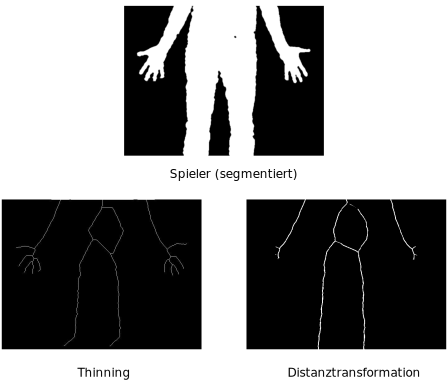
\includegraphics[width=1.0\linewidth]{./fig/vergleich-screenshot0}
\caption{}
\label{fig:vergleich-screenshot0}
\end{figure}
Abbildung \ref{fig:vergleich-screenshot12} zeigt ebenfalls deutliche Unterschiede in den Skeletten. Auffallend sind die Lücken in den Skelettlinien des Skeletts, das aus der Distanztransformation entstanden 
ist. Der Thinning-Algorithmus hat stets ein Skelett mit zusammenhängenden Skelettkomponenten als Ergebnis. 
Jedoch ist beim Skelett des Thinning-Algorithmus ein Ausläufer zu erkennen, der nicht die eigentliche Form
des Objektes beschreibt. Das aus der Distanztransformation resultierende Skelett gibt den Oberkörper bis
zu den Schultern als eine Linie ohne Ausläufer wieder.\\
Eine weitere Eigenschaft einer Skelettlinie ist ihre Breite, die sich idealerweise auf einen Pixel beschränkt. Dies ist beim Thinning der Fall, bei der Distanztransformation fällt die Skelettlinie breiter
aus. Wird das Skelett zur Datenkomprimierung genutzt, enthalten unnötige Pixel mehr Informationen, als 
eigentlich benötigt wird. Für andere Anwendungen muss diskutiert werden, ob eine 1-Pixel-Breite unbedingt erfüllt sein muss.\\
\begin{figure}[htbp]
\centering
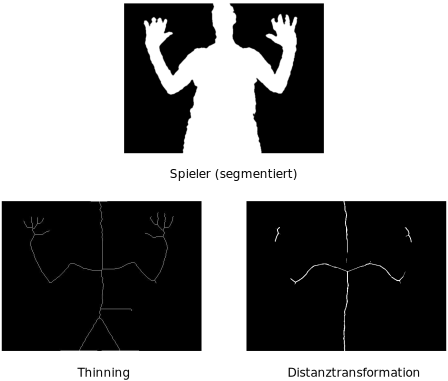
\includegraphics[width=1.0\linewidth]{./fig/vergleich-screenshot12}
\caption{}
\label{fig:vergleich-screenshot12}
\end{figure}
Bezüglich der Skelettqualität liefert der Thinning-Algorithmus sehr
gute Skelette. Hier sind keine weiteren Verbesserungen mehr nötig.
Bei dem Distanzskelett sind Verbesserungen, besonders bei der 
Konnektivität des Skelettes, möglich. In Abschnitt \ref{sec:verbesserung} stellt zwei Verbesserungsmöglichkeiten vor.
\section{Laufzeiten}
Die Laufzeit wurde mit dem Profiling-Tool \emph{CProfile} gemessen. Es erstellt für Python-Programme eine Statistik über die Laufzeiten eines Programms und seine einzelnen Funktionen. Es wurde jeweils eine Statistik
für die Implementierung des Thinning-Algorithmus und des Algorithmus der Distanztransformation erstellt. Die
wichtigsten Funktionen der Programme wurden aus der Statistik entnommen. Die Tabellen \ref{tab:laufzeiten_distanztransformation} und \ref{tab:laufzeiten_thinning} geben einen
Überblick über die Laufzeiten. \\
Obwohl der Thinning-Algorithmus bezüglich der gewünschten Eigenschaften von Skeletten die besten Ergebnisse
liefert, ist er deutlich langsamer als die Skelettierung mittels
Distanztransformation. Diese nimmt etwa $60\%$ der Gesamtlaufzeit
des Programms ein, während die Skelettierung nach Thinning etwa
$92\%$ der gesamten Programmlaufzeit beansprucht.
\begin{table}[htbp]
\begin{center}
\begin{tabular}{|c|c|c|c|}
 \hline
  \multicolumn{4}{|c|}{46371 Funktionsaufrufe in 16.723 CPU-Sekunden} \\
  \hline
\hline 
\textbf{Funktion} & \textbf{Anzahl Aufrufe} & \textbf{Gesamtzeit} [$s$] & \textbf{Pro Aufruf} [$s$]\\ 
\hline Startfunktion & 126 & 16.723 & 16.723 \\ 
\hline Spielersegmentierung & 126 & 0.453 & 0.004  \\ 
\hline Berechnung des Distanzskeletts & 126 & 9.594 & 0.076    \\ 
\hline 
\end{tabular} 
\end{center}
\caption{Laufzeiten Skelettierung mittels Distanztransformation}
\label{tab:laufzeiten_distanztransformation}
\end{table}
\begin{table}[htbp]
\begin{center}
\begin{tabular}{|c|c|c|c|}
 \hline
  \multicolumn{4}{|c|}{1424 Funktionsaufrufe in 28.159 CPU-Sekunden} \\
  \hline
\hline 
\textbf{Funktion} & \textbf{Anzahl Aufrufe} & \textbf{Gesamtzeit} [$s$] & \textbf{Pro Aufruf} [$s$]\\
\hline Startfunktion & 29 & 28.159 & 28.159 \\ 
\hline Spielersegmentierung & 29 & 0.088 & 0.003  \\ 
\hline Berechnung des Distanzskeletts & 29 & 26.224 & 0.904    \\ 
\hline 
\end{tabular} 
\end{center}
\caption{Laufzeiten Skelettierung mittels Thinning}
\label{tab:laufzeiten_thinning}
\end{table}
\newpage
\section{Distanztransformation - Verbesserung der Skelettqualität}
\label{sec:verbesserung}
Im Folgenden wird ein Ansatz zur Verbesserung der Skelettqualität
vorgestellt. Dieser ist außerhalb der offiziellen Projektarbeit
entstanden. \\
Das Skelett, welches mit der Methode der Distanztransformation bestimmt wurde, weist Lücken zwischen den Skelettteilen auf. Um die Topologie und geometrische Eigenschaften des Objekts gut wiederzugeben, ist ein lückenloses Skelett wünschenswert. \\
Die Ursache der Lücken ist die Segmentierung des Gradientenbetrages der Distance Map. Dies wird anhand von Abbildung \ref{fig:person-skelett} deutlich. Im Gradientenbild (Teilabbildung b) sind noch durchgehende Skelettlinien zu erkennen. Per Schwellwert-Filter wird das Skelett aus dem Gradientenbild extrahiert. Für das gezeigte Beispielbild konnte allerdings kein geeigneter Schwellwert gefunden werden, der sowohl Pixelkonnektivität gewährleistet als auch Artefakte verhindert. Teilabbildung c zeight die Segmentierung des Gradientenbildes. In diesem Schritt ist die Pixelkonnektivität erstmals nicht gewährleistet. Auch in den folgenden Schritten wird die Pixelkonnektivität nicht wieder hergestellt. 
\begin{figure}[htbp]
\centering
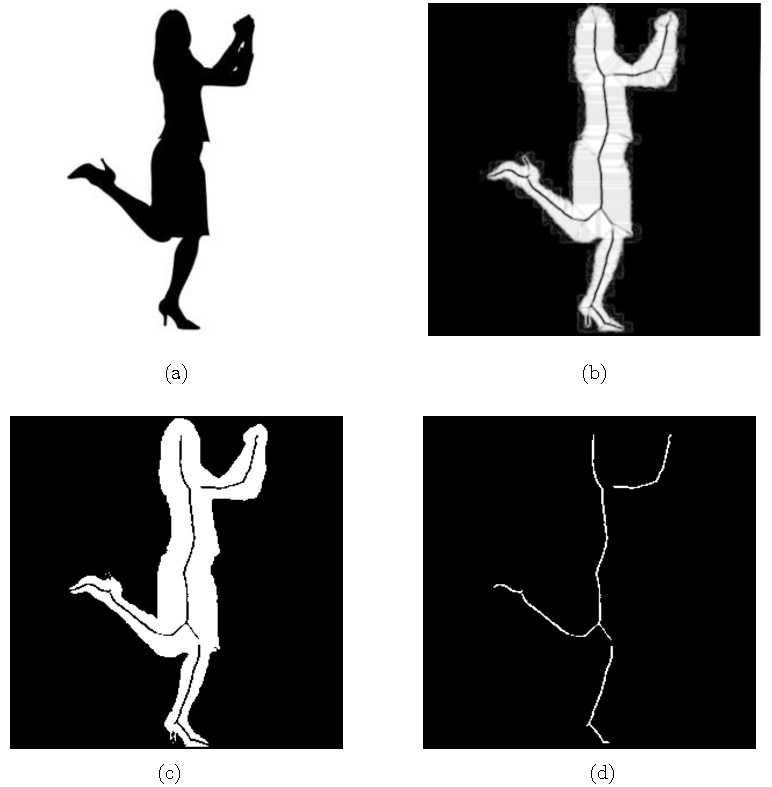
\includegraphics[width=1.0\linewidth]{./fig/person_gradienten_problem.pdf}
\caption{Bestimmung des Skelett mittels Distanztransformation. (a) Originalbild (b) Gradientenbild (c) Gradientenbild segmentiert(d) Skelett}
\label{fig:person-skelett}
\end{figure}\\
In den folgenden Abschnitten werden Methoden zur Verbesserung des Skeletts vorgestellt. Dies umfasst zum einen die Herstellung Konnektivität der Skelettkomponenten beziehungsweise dem Füllen der Lücken zwischen den Skelettlinien. Zum anderen ist es wünschenswert, dass die Skelettlinie des Objektes nicht breiter als ein Pixel ist. Zuerst wurden markante Punkte auf dem Skelett bestimmt. Diese wurden
genutzt, um mittels Breitensuche oder Tiefensuche Pfade zwischen ihnen zu finden und sie zu verbinden. Punkte werden miteinander
verbunden, wenn sie nah genug beieinander sind. Das Ergebnis ist ein Skelett mit
zusammenhängenden Skelettlinien. 
\subsection{Berechnung von Features auf dem Skelett}
\label{subsec:features}
Die Bildverarbeitungsbibliothek \emph{OpenCV} bietet Funktionen zur Bestimmung von markanten Punkten, sogenannten \emph{Features},
in einem Bild. Die Funktion \texttt{goodFeaturesToTrack} bestimmt die stärkesten Ecken in einem Bild oder Bildausschnitt nach einem Algorithmus von \cite{goodfeatures}. Mittels eines Qualitätsmaßes wird entschieden, ob die Stärke einer
Ecke an einem bestimmten Pixel ausreicht, um in die Featuremenge aufgenommen zu werden. Für die
Funktion können der Wert des Qualitätsmaßes, den eine Ecke erfüllen muss, die Anzahl der Ecken, die gefunden werden sollen und die
minimale Distanz zwischen den stärksten Ecken übergeben werden.\\
Die Qualität einer Ecke wird anhand von Eigenwerten bestimmt. Die Eigenwerte beziehen sich dabei auf 
die Kovarianzmatrix von Ableitungen einer festgelegten Umgebung eines Pixels. Es wird minimale Eigenwert
für die Eckendetektion weiterverwendet. Ist der minimale Eigenwert einer Ecke kleiner als das gewünschte
Qualitätsmaß, wird diese Ecke verworfen. Die verbleibenden Ecken werden nach ihrer Qualität absteigend sortiert. Anschließend wird überprüft, ob es in der spezifizierten Distanz Ecken gibt, die stärker sind. 
\begin{figure}[htbp]
\centering
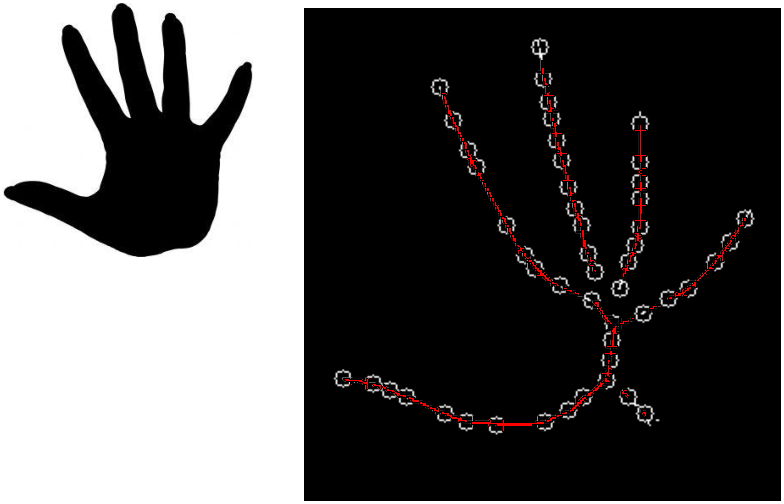
\includegraphics[width=0.7\linewidth]{./fig/features.pdf}
\caption{Ergebnis der Funktion \texttt{goodFeaturesToTrack}. Links: Originalbild. Rechts: Berechnetes Distanzskelett mit Features. Die roten Linien markieren das Rohskelett, die weißen Kreise markieren die Features, die auf dem Skelett gefunden wurden.}
\label{fig:features}
\end{figure}
Abbildung \ref{fig:features} zeigt das Ergebnis der Berechnung. Die Kreise markieren die Feature-Punkte. Wie man erkennen kann, befinden sich die Features auf der Skelettlinie. Dies ist hilfreich für die weiteren
Verbesserungen des Skeletts. Befinden sich Features außerhalb der Skelettlinien könnten die ursprüngliche Form des Skeletts und die Topologie des Objekts verfälscht werden.
\subsection{Breitensuche}
\label{subsec:breitesuche}
Der Breitensuche-Algorithmus durchsucht einen Graphen ausgehend von einem Startpunkt nach weiteren 
Knoten. Der Algorithmus sucht zunächst nur nach direkt nachfolgenden Knoten und somit in die Breite des
Graphen. Knoten, die bereits besucht wurden, werden markiert. Wurde ein Knoten noch nicht besucht, wird er
in eine \emph{Queue} (Warteschlange) aufgenommen.\\
Mittels Breitensuche sollen Pfade zwischen den markanten Punkten auf dem Skelett gefunden werden. Die markanten Punkte entsprechen Knoten in einem Graphen. Für die Nachbarschaftsbeziehung zwischen zwei
Knoten wird ein Nachbarschaftsmaß definiert. Abbildung \ref{fig:suchdistanz_naechster_nachbar} zeigt, wie überprüft wird, ob ein Punkt in einem festgelegten Intervall des Punktes $(x,y)$ liegt. Es wird eine Suchdistanz für beide Richtungen festgelegt. Sie
wird entsprechend der minimalen Distanz, die zwischen markanten Punkten erlaubt ist, gewählt (Abschnitt \ref{subsec:features}). \\
Erst wird in x-Richtung gesucht, dann in y-Richtung. Fällt der Punkt in das Intervall, wird er als besucht markiert und
mit dem Punkt $(x,y)$ verbunden. 
In Anhang \ref{anhang:quellcode} befindet sich der Quellcode zur Breitensuche. Die Zeilen $78$/$79$ von Listing \ref{lst:breitensuche} zeigen die Umsetzung des Suchkreuzes aus der Abbildung. 
\begin{figure}[htbp]
\centering
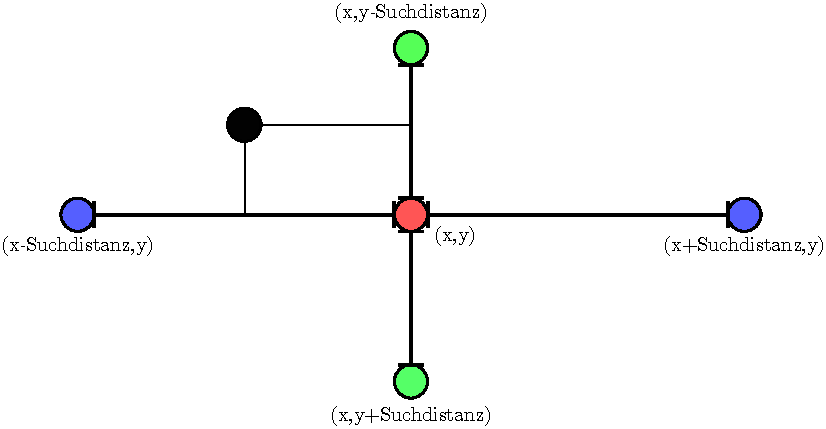
\includegraphics[width=1.0\linewidth]{./fig/suchdistanz_naechster_nachbar}
\caption{Das aufgespannte Suchkreuz vom Punkt $(x,y)$ (rot) aus. Für den schwarzen Punkt wird überprüft, ob er in den festgelegten Suchintervallen des Punktes $(x,y)$ liegt.}
\label{fig:suchdistanz_naechster_nachbar}
\end{figure}\\
Das Ergebnis des Algorithmus ist in Abbildung \ref{fig:hand_BFS} im Vergleich zum vorigen Skelett zu sehen.
Das Skelett besitzt nun zusammenhängende Komponenten. Auffällig sind die Ausläufer, die auf die 
Vorgehensweise des Breitensuchealgorithmus zurückzuführen sind. Wird die Suchdistanz zu groß gewählt,
findet der Algorithmus mehrere Nachfolger, die er dann mit dem aktuellen Punkt verbindet. Das Ergebnis
sind fächerartige Ausläufer.
\begin{figure}[htbp]
	\centering
	\begin{minipage}{5cm}
		\centering
		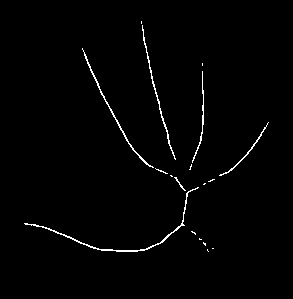
\includegraphics[width=1.0\linewidth]{./fig/hand-skelett}
	\end{minipage}
	\hspace{2cm}
	\begin{minipage}{5cm}
		\centering
		
\includegraphics[width=1.0\linewidth]{./fig/hand-bfs}
	\end{minipage}
	\caption{Ergebnis der Breitensuche.}
	\label{fig:hand_BFS}
	\end{figure}
\subsection{Tiefensuche}
\label{subsec:tiefensuche}
Wie bei der Breitensuche wird ausgehend von einem Startknoten ein Graph nach weiteren Knoten durchsucht. 
Im Gegensatz zur Breitensuche erfolgt das Traversieren des Graphens in die Tiefe. Wurde ein Nachfolgeknoten
gefunden, wird für diesen weiter geprüft, ob er ebenfalls einen Nachfolgeknoten besitzt. Dies wird
solange wiederholt (rekursiv) bis kein Nachfolgeknoten mehr gefunden werden kann. Mittels \emph{Backtracking} wird der Pfad zurückverfolgt. Anschließend wird ein neuer Knoten als Startpunkte gesucht, der noch nicht besucht wurde und das Durchsuchen nach nächsten Nachbarn wird für diesen Knoten wiederholt.\\
Die Suche nach dem nächsten Nachbarn funktioniert wie bei der Breitensuche (Abbildung \ref{fig:suchdistanz_naechster_nachbar}). \\
Das Ergebnis ist in Abbildung \ref{fig:hand_DFS} zu sehen. Es fällt auf, dass es noch Lücken im Skelett gibt, was auf die Suchdistanz zurückzuführen ist. Ist sie zu klein, können keine weiteren Punkte im Umkreis des aktuellen Punktes gefunden werden und der Algorithmus endet für diesen Pfad. 
\begin{figure}[htbp]
	\centering
	\begin{minipage}{5cm}
		\centering
		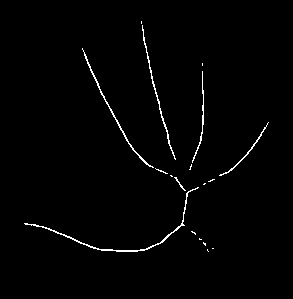
\includegraphics[width=1.0\linewidth]{./fig/hand-skelett}
	\end{minipage}
	\hspace{2cm}
	\begin{minipage}{5cm}
		\centering
		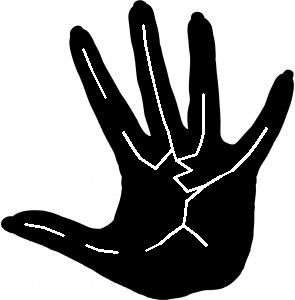
\includegraphics[width=1.0\linewidth]{./fig/hand-dfs}
	\end{minipage}
	\caption{Ergebnis der Tiefensuche.}
	\label{fig:hand_DFS}
	\end{figure}\\
Um die Konnektivität des Skeletts zu gewährleisten, muss das Skelett nachbearbeitet werden. \\
Das Skelett, welches aus der ersten Stufe der Verbesserung entstanden ist, besitzt Zusammenhangskomponenten. Innerhalb der Zusammenhangskomponenten ist die Pixelkonnektivität gewährleistet, die globale Konnektivität zwischen den Komponenten jedoch nicht. Die Idee des
nächsten Verbesserungsschrittes ist es, die Zusammenhangskomponenten
zu verbinden, die am nächsten beieinander liegen. Dazu werden
die Punkte aus den Zusammenhangskomponenten extrahiert, die die Endpunkte der Komponenten sind. Das sind
entweder Punkte ohne Vorgänger oder ohne Nachfolger. 
Für diese Punkte wird der nächste Nachbarpunkt bestimmt, der
ebenfalls ein Endpunkt einer Komponente ist. Zwischen den Endpunkten der aktuell betrachteten Komponente und den Endpunkten anderer Komponenten wird der euklidischen Abstand bestimmt und der Punkt als nächsten Nachbar gewählt, der den minimalen Abstand zu dem fest gewählten Punkt hat. Wichtig ist, dass nur Punkte
verbunden werden, die jeweils auf unterschiedlichen Zusammenhangskomponenten liegen. Welcher Punkt auf welcher Komponente liegt, wird bereits bei der Tiefensuche bestimmt. 
In Abbildung \ref{fig:offeneenden} wurden die Endpunkte farbig markiert. Dies sind
alles Kandidaten zum Verbinden der Komponenten. Das Skelett besitzt in dieser Abbildung fünf Zusammenhangskomponenten,
wobei eine Zusammenhangskomponente aus genau einem Punkt besteht
(auf dem Ringfinger der Hand). Dieser Punkt besitzt weder einen Vorgänger noch einen Nachfolger.
\begin{figure}[h!]
\centering
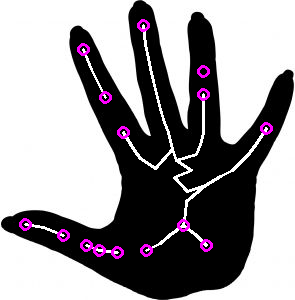
\includegraphics[width=0.4\linewidth]{./fig/offeneEnden.png}
\caption{Zusammenhangskomponenten und ihre Endpunkte.}
\label{fig:offeneenden}
\end{figure}
\begin{figure}[h!]
\centering
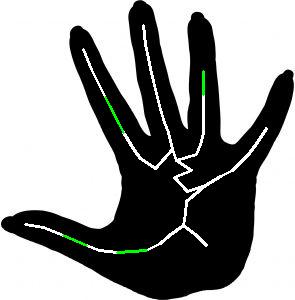
\includegraphics[width=0.4\linewidth]{./fig/dfs-endergebnis-hand2.png}
\caption{Ergebnis des zweiten Verarbeitungsschrittes der Tiefensuche. Die weiße Linie ist das Skelett,
das aus dem ersten Verarbeitungsschritt entstanden ist. Die grünen
Linien sind die Verbindungen zwischen den Zusammenhangskomponenten.}
\label{fig:hand-DFS-endergebnis}
\end{figure}
Abbildung \ref{fig:hand-DFS-endergebnis} zeigt, wie die Zusammenhangskomponenten miteinander verbunden
wurden. Es wurden immer die Zusammenhangskomponenten miteinander verbunden, die sich am nächsten liegen.
Nun ist die Skelettkonnektivität gegeben.
\section{Fazit}
Beide Algorithmen (Thinning und Distanztransformation) liefern 
Skelette. Diese realisieren die gewünschten Eigenschaften eines
Skeletts. Dabei ist die Skelettqualität unterschiedlich. Der
Thinning-Algorithmus liefert bezüglich Pixelkonnektivität, 
1-Pixel-Breite und Wiedergabe der Topologie hervorragende Ergebnisse. Bei der Skelettierung mittels Distanztransformation
ist vor allem auffällig, dass die Pixelkonnektivität nicht vollständig gegeben ist. \\
Es wurden Verbesserungsmöglichkeiten diskutiert, die auch zur globalen Pixelkonnektivität bei einem Distanzskelett führen. 
Da es sich um einen Ansatz handelt, der nach der Projektzeit 
entstanden ist, wurde der Ansatz nicht auf der Kinect, sondern auf
statischen Bildern getestet. \\
Laufzeit...